\section{引言}

\CJKindent LED\footnote{Light Emitting Diode} 是发光二极管的简称。九十年代白光 LED 的研制成功,为照明产业开辟了一项全新的技术领域。该领域技术发展迅速应用面广产业带动性强,节能潜力大,被各国公认为最有发展前景的高技术节能产业之一。由于LED的低电压、低电流,因而白光LED发热量低,耗电最小。这种固体光源具有耐震动、抗冲击、长寿命和无污染等独特的优点。本文从白光LED的发光机理,LED芯片设计以及大功率LED的设计等方面进行了深入的探讨。

\section{LED发光原理}

\CJKindent LED发光二极管不但具有一般PN结的电学特性,即正向导通,反向截止、击穿特性。此外,在一定条件下,它还具有发光特性。

\CJKindent 如图\ref{led1}所示,LED加正向电压后,电子由N区注入P区,空穴由P区注入N区。进入对方区域的少数载流子(少子)一部分与多数载流子(多子)复合而发光。能源源不断地从相对的方向将大量的多数空穴载流子与大量的多数电子载流子分别注入PN结,大量的空穴.电子载流子在PN结中复合时会把多余的能量以光的形式释放出来,从而把电能直接转换为光能。这种利用注入载流子的电致发光原理制作的二极管叫发光二极管,通称LED。当电流从LED阳极(P区)流向阴极(N区)时,半导体晶体就发出从紫外到红外不同颜色的光线,光的颜色与LED的晶体材料种类有关,光的强弱与电流强度有关。
\begin{figure}[h]
\centering
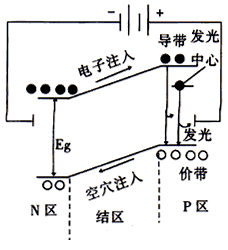
\includegraphics[scale=1]{led1}
\caption{LED发光原理}
\label{led1}
\end{figure}

\section{白光LED实现方式}
\begin{enumerate}
\item 多芯片组合

\CJKindent 光色混合型白光LED是指多芯片(n ≥ 2)组合复合成的白光LED器件。具有能量损耗少、发光效率高的优点。并且显色性便于调节和改善,可以获得高显色指数。缺点是设计复杂、电路控制困难、成本较高。

\item 荧光体转换白光 LED
\begin{enumerate}
\item 近紫外 LED + RGB 荧光粉\cite{powerled1}

	\CJKindent 采用高亮度的近紫外 LED 泵浦 RGB 三色荧光粉, 产生红、绿、蓝三基色。通过调整三色荧光粉的配比可以形成白光。相对于蓝光 LED + YAG 荧光粉, 采用这种方法更容易获得颜色一致的白光。近紫外 LED 光谱如图\ref{fluoled2}所示。

\begin{figure}[h]
\centering
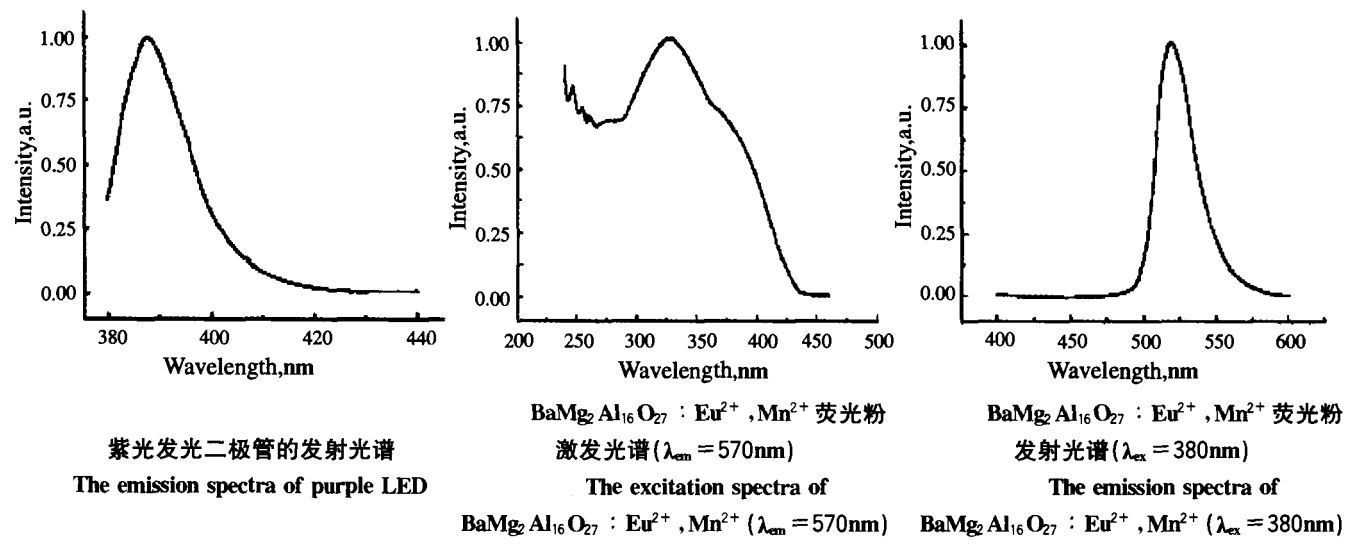
\includegraphics[scale=0.3]{fluoled2}

\caption{近紫外 LED \label{fluoled2}}
\end{figure}

\CJKindent 国内外最新研制的近紫外 InGaN LED发光波长在 380nm 左右,有研稀土新材料股份有限公司研发了一系列近紫外LED用三基色荧光粉,也有报道提出了用近紫外LED激 发白色荧光粉 ZnS : Ag、CdZnS : Cu, AI 得到白光\cite{fluoled}。

\item 蓝光 LED + YAG 荧光粉

	\CJKindent 以功率型 GaN 基蓝光 LED 为泵浦源, 激发黄色无机荧光粉或黄色有机荧光染料, 由激发获得的黄光与原有蓝光混合产生视觉效果的白光。蓝光 LED 发光光谱如图\ref{fluoled3}所示。

\begin{figure}[h]
\centering
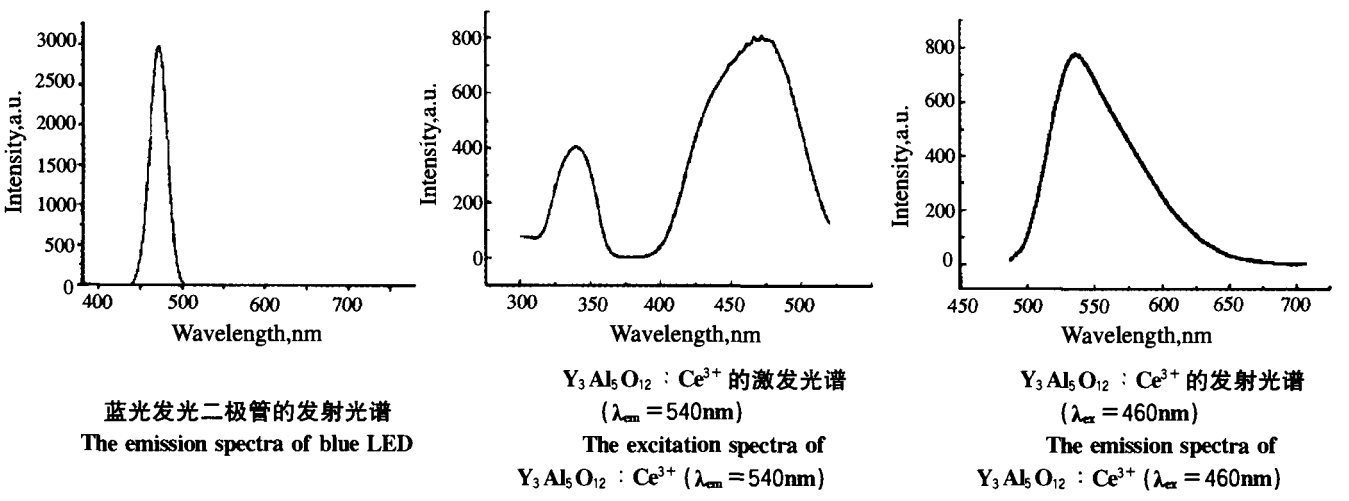
\includegraphics[scale=0.3]{fluoled3}

\caption{蓝光 LED \label{fluoled3}}
\end{figure}

\CJKindent 当今使用最多的蓝光 LED是 InGaN 蓝光LED,发射峰值 450-480nm\cite{fluoled}。

\end{enumerate}
\item 非荧光转换的白光 LED\cite{powerled2}

	\CJKindent 利用 ZnSe 产生白光的技术。在 ZnSe 单晶基板上形成 CdZnSe 薄膜,通电后使薄膜发出蓝光,同时部分蓝光照射到基板上而发出黄光,最后蓝光黄光混合后形成白光。

\item 量子点白光 LED \cite{powerled2}

	\CJKindent 分为以下四种方式:
	\begin{enumerate}

\item 利用量子点表面缺陷态发光得到白光 LED

	\item 利用单源二色互补得到白光 LED

	\item 利用三基色量子点得到白光 LED

	\item 利用蓝紫光 LED 与量子点荧光粉组合得到白光 LED

	\end{enumerate}

\section{提高量子效率的措施\cite{powerled2}}
\item 提高内部量子效率
\begin{enumerate}
	\item 用异质结构代替同质结构
	\item 采用量子阱做活性层
\end{enumerate}

	\item 提高外部量子效率
\begin{enumerate}
	\item 换为透明衬底或在有吸收功能的衬底上加反射镜(反射镜一般采用高反光金属材料如 AL 和 Ag)。
	\item 采用半圆形球面(一般 LED 光因临界角被限制而不易射出,做成半圆形球面使光不受临界角限制)。
	\item 表面采用织状结构或粗糙面以增加光的射出面。
	\item 改变几何形状(一般 LED 为平面正方形长方形结构,此些结构容易制造但限制了光的输出)。如改成漏斗形后光更容易的输出。
	\item 采用光子晶体。光子晶体对光子的控制正如半导体对电子一样。半导体中能量落在禁带中的电子不能传输。同理光子晶体中的周期性结构使之产生能带结构,能量在光带隙中的光子同样不能被传输,只能被射出。可以控制光射出使产生的光子在某些模态内加强而另一些模态内被压制所以在光子晶体中,有一些能量的光子不能够穿透晶体而被反射出,此种现象可以被用作增强 LED 的光输出。
\end{enumerate}


\section{大功率LED芯片的发展趋势\cite{powerled1}}
\begin{enumerate}

\item 基于功率型高效蓝光和紫外 LED 芯片的半导体照明光源

\item 芯片结构的改进 : 倒装焊 ( Flip-chip ) 结构

\begin{figure}[H]
\centering
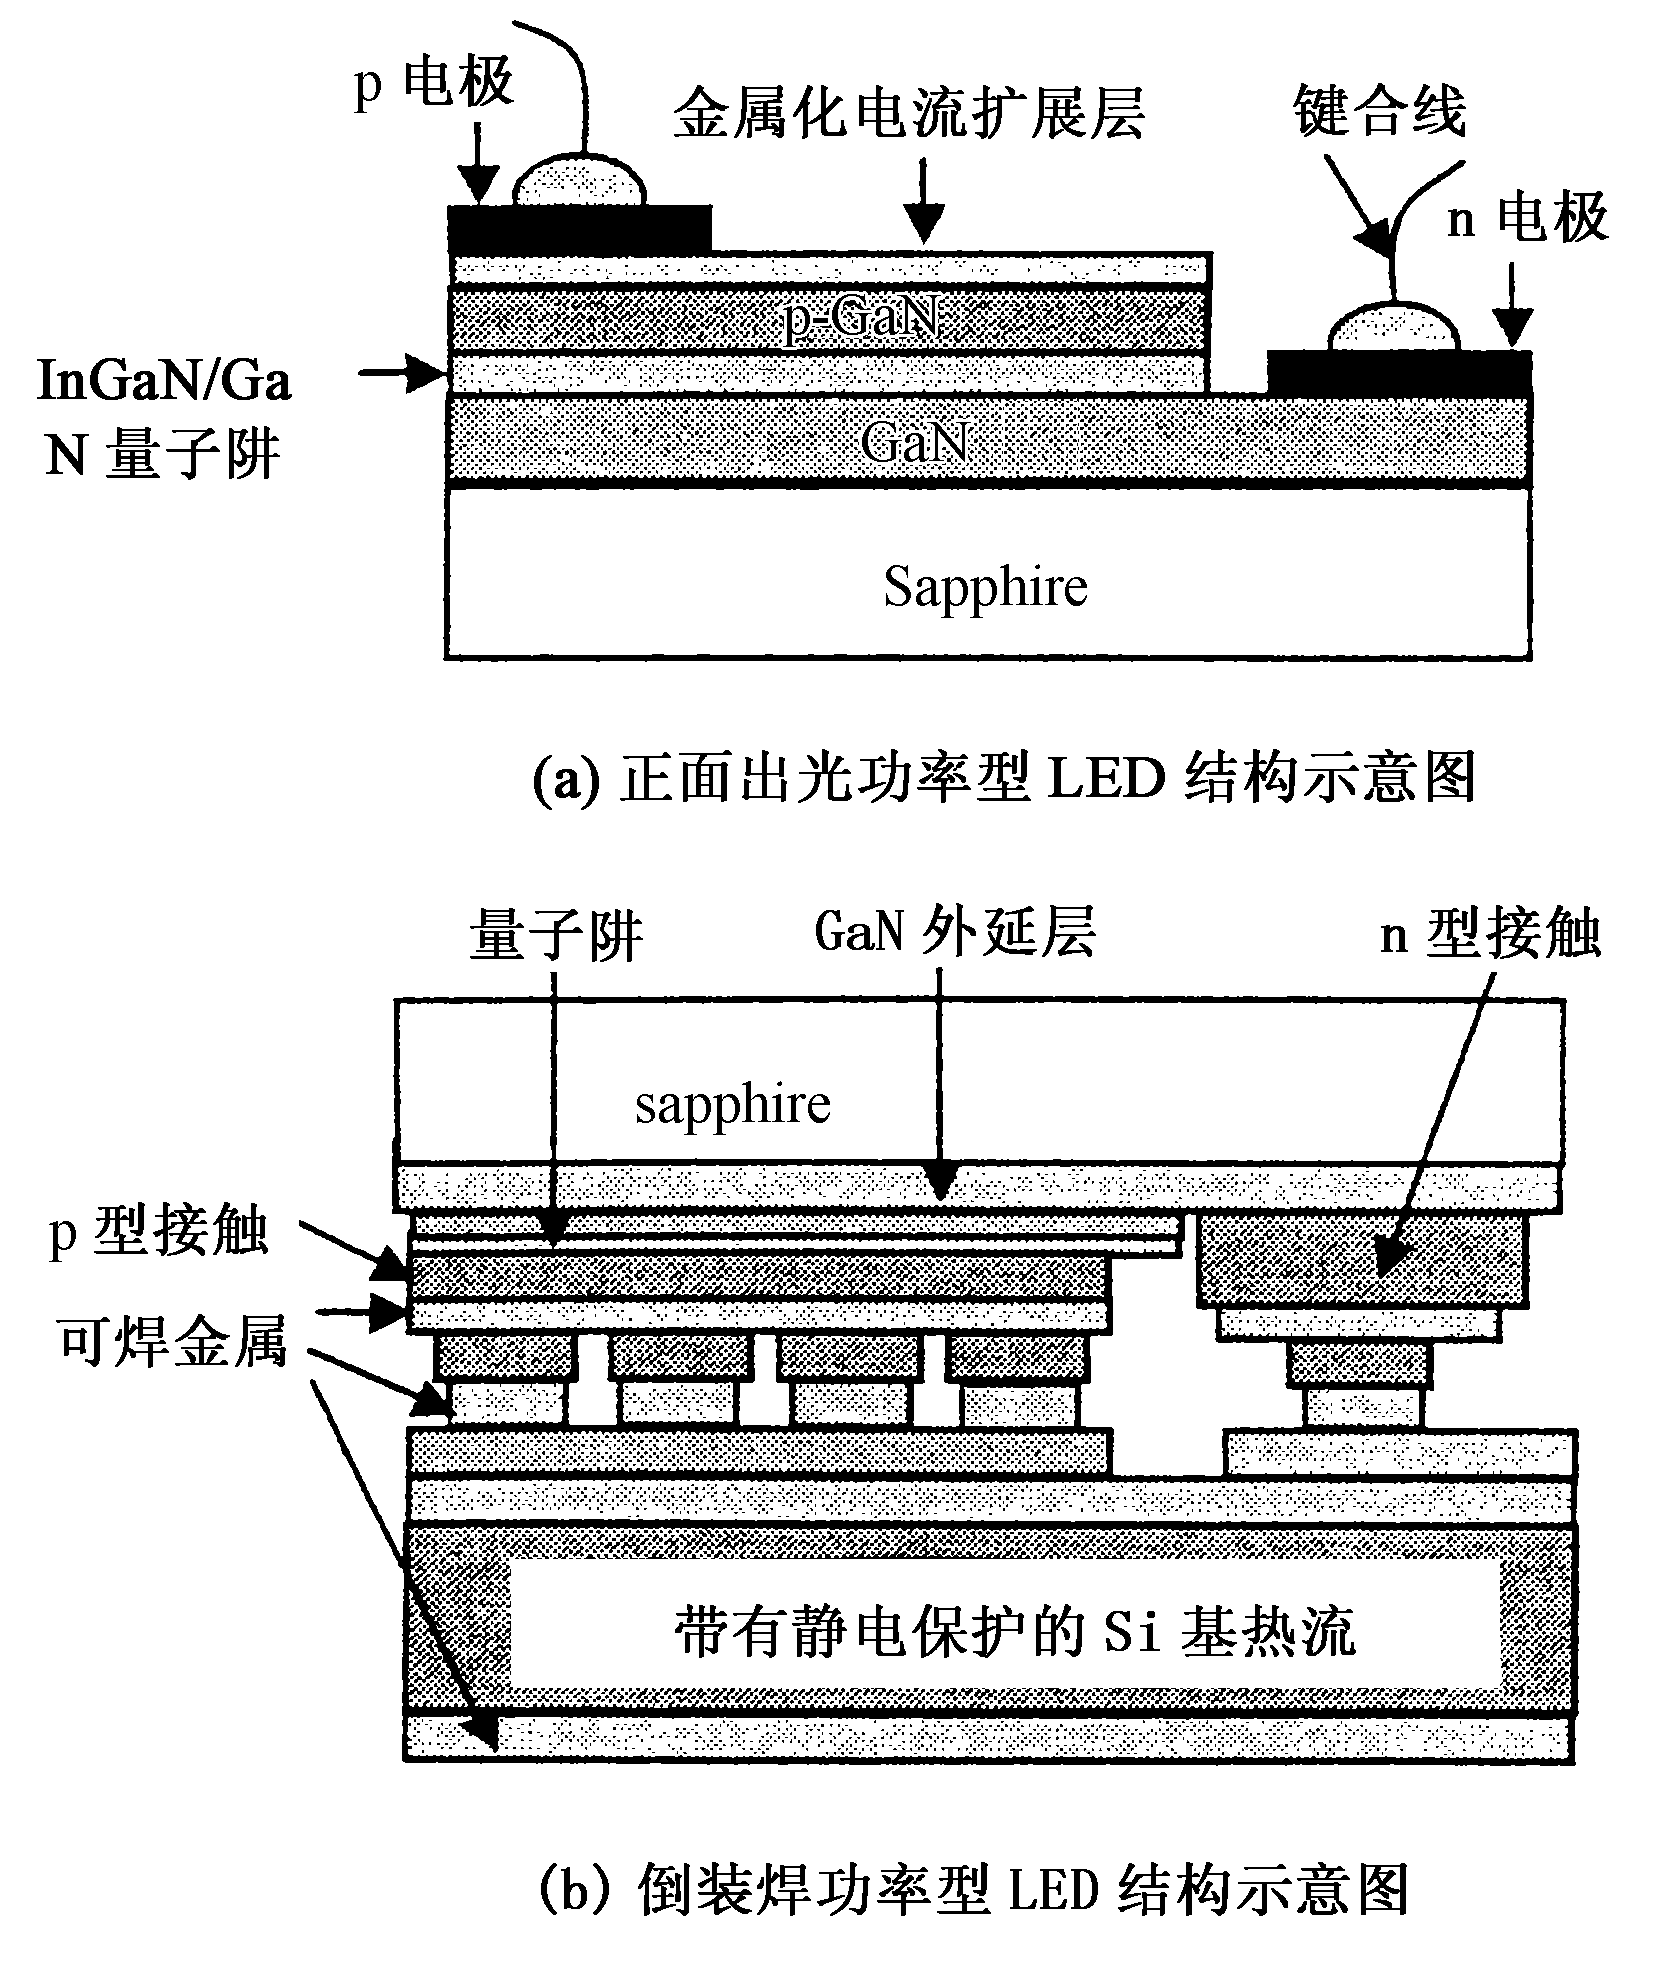
\includegraphics[scale=0.2]{led3.png}
\caption{倒装焊结构}
\label{led3}
\end{figure}

\end{enumerate}

\end{enumerate}

%===========参考文献===========
\newpage
\bibliography{bibfile}
%==============================

